\documentclass[tikz,border=8pt]{standalone}
\usepackage{amsmath}
\usetikzlibrary{arrows.meta,decorations.pathreplacing}
\begin{document}

% Asset ID: AS2DataPresentationTikZ-006
% Source: Width and height of bars evidence.
% Related lesson section: Worked Examples 15 and 16.
% Purpose: Use a known bar to scale drawn width and height.
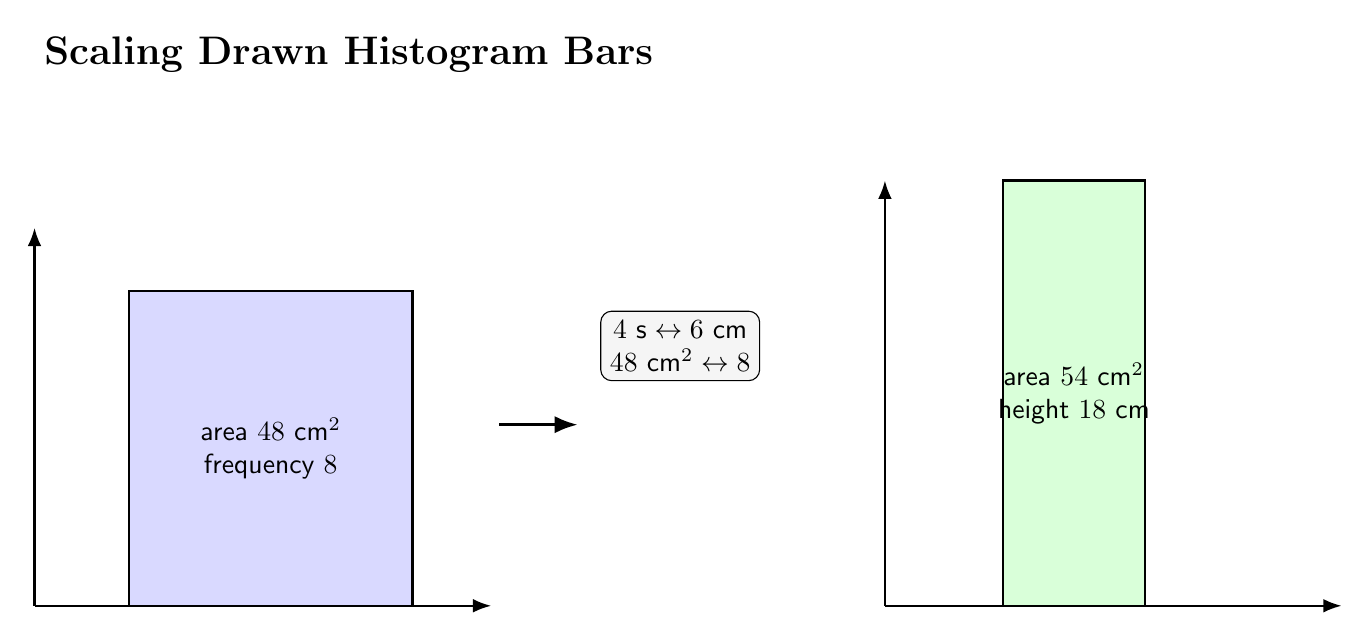
\begin{tikzpicture}[>=Latex,font=\sffamily]
\node[anchor=west,font=\bfseries\Large] at (0,8.0){Scaling Drawn Histogram Bars};
\draw[->,thick] (0,1)--(5.8,1); \draw[->,thick] (0,1)--(0,5.8); \draw[fill=blue!15,thick] (1.2,1) rectangle (4.8,5.0);
\node[align=center] at (3,3){area $48\text{ cm}^2$\\frequency $8$};
\node[draw,rounded corners,fill=gray!8,align=center] at (8.2,4.3){$4\text{ s}\leftrightarrow6\text{ cm}$\\$48\text{ cm}^2\leftrightarrow8$};
\draw[->,very thick] (5.9,3.3)--(6.9,3.3);
\draw[->,thick] (10.8,1)--(16.6,1); \draw[->,thick] (10.8,1)--(10.8,6.4); \draw[fill=green!15,thick] (12.3,1) rectangle (14.1,6.4);
\node[align=center] at (13.2,3.7){area $54\text{ cm}^2$\\height $18\text{ cm}$};
\end{tikzpicture}

\end{document}
